\chapter{ERCOT: The Energy-Only Grid}
\label{ch:ercot}

The previous chapter treated the grid as a machine. This chapter treats it as a market, and one market in particular: ERCOT, the Electric Reliability Council of Texas, where more Bitcoin mining load is connected than anywhere else in the world. Everything in Parts II and III of this book (breakeven prices, curtailment strategies, ancillary services, transmission charges) plays out inside the market rules described here.

\section{From Monopolies to Markets}

For most of the twentieth century, electricity in the United States was delivered by \glossaryterm{vertically-integrated-utility-monopoly}{vertically integrated utility monopolies}: in each region, a single company owned the power plants, the wires, and the relationship with every customer \autocite{EPAMarketStructure}. Regulators, not markets, set the prices. State Public Utility Commissions approved investments and granted the utility an allowed rate of return; consumers had no choice of supplier.

Starting in the 1990s, federal policy pried this model open. FERC Order No.\ 888 (1996) required utilities to open their transmission lines to third-party generators on non-discriminatory terms, and Order No.\ 2000 (1999) encouraged the voluntary formation of \glossaryterm{regional-transmission-organization}{Regional Transmission Organizations} (RTOs): neutral, non-profit operators that run the grid and administer wholesale markets across multi-state regions \autocite{ferc1996order888,ferc1999order2000}. % src: Order 888 issued Apr 24, 1996; Order 2000 issued Dec 20, 1999 (89 FERC 61,285); verified from FERC pages/order PDF
Generation became a competitive business. Independent power producers could build plants and sell into open markets, and in many states consumers gained the right to choose their retail supplier. Today roughly two-thirds of U.S. electricity consumers live in regions where the transmission system, and the wholesale market on top of it, is run by these \glossaryterm{independent-system-operator}{Independent System Operators} (ISOs) and RTOs \autocite{EPAMarketStructure}; % src: EPA page (updated Jul 2026): "About two-thirds of U.S. electricity consumers live in a region where transmission is managed by an ISO or RTO"
 the rest remain under traditional regulated monopolies. ISOs and RTOs own no generation and serve no retail customers themselves. They dispatch generators, operate the transmission system, and run the auctions where electricity is bought and sold, which keeps them neutral among the competitors whose power they move.

Seven such markets serve most U.S. electricity consumers \autocite{isorto2026home}. % src: isorto2026home ("Ten ISOs/RTOs serve two-thirds of electricity consumers in the United States"; the seven U.S. ones are CAISO, ERCOT, ISO-NE, MISO, NYISO, PJM and SPP); until 2026-10-12 this said "cover most of the country", which is not true by area (review suggestion)
This book concerns itself with exactly one of them.

\section{The Island Grid}

ERCOT operates the Texas Interconnection introduced in Chapter~2: one of the three synchronous grids in the continental United States, and by far the smallest. It serves about 90~percent of Texas electric load, more than 27 million customers \autocite{ercot2026factsheet}. % src: ERCOT Fact Sheet, Aug 2026: "more than 27 million Texas customers, representing about 90 percent of the state's electric load"
Its isolation is deliberate. Because its wires stay (almost) entirely inside Texas, ERCOT's wholesale market is exempt from FERC rate regulation (federal reliability standards still apply), an arrangement Texas has defended since the 1930s \autocite{ercot2025gridinsightsabout}. % src: ERCOT Grid Insights, Nov 2025: "exempt from wholesale regulation by FERC... subject to FERC oversight through NERC's Reliability Standards"
The connections that do exist are three DC ties and one variable-frequency transformer, about 1,220~MW in total: 820~MW toward the Eastern Interconnection and 400~MW toward Mexico, less than two percent of ERCOT's peak demand \autocite{ercot2025gridinsightsdcties}. % src: ERCOT Grid Insights, May 2025: SPP ties 820 MW (North 220 + East 600), Mexico 400 MW (Railroad 300 + Laredo VFT 100); 1,220/91,200 (ERCOT's all-time peak demand, July 22, 2026; see ch8 sec:fourcp-peaks) = 1.3%
Isolation limits outside support and gives Texas autonomy over its market design. Chapter~2 showed that limit during Winter Storm Uri. Texas restructured its market on its own terms with Senate Bill 7 (1999), opening retail choice from January 2002, and it can change its market design without federal proceedings \autocite{texas1999sb7}. % src: Tex. Util. Code sec. 39.102(a), enacted by S.B. 7, 76th Leg. (1999); full retail competition from Jan 1, 2002

For a large electricity consumer, ERCOT's isolation also means operating entirely inside ERCOT's pricing system and market rules, with ERCOT as the only grid operator.

\section{An Energy-Only Market}

Most U.S. markets pay generators twice: once for the energy they produce, and once, through a \glossaryterm{capacity-market}{capacity market}, for simply existing and promising to be available years into the future. ERCOT does not. It is an \glossaryterm{energy-only-market}{energy-only market}: a generator earns money by selling energy and ancillary services, and nothing else \autocite{ercot2025gridinsightsabout}. If those revenues do not justify building a power plant, the plant does not get built.

If generators must recover their investment from energy prices alone, then prices during scarcity must be allowed to rise very high; those few expensive hours are what pay for the capacity that sits idle the rest of the year. ERCOT's price cap, and the mechanism that pushes prices toward it, are covered in Section~\ref{sec:ordc}. The same design is what makes ERCOT interesting for flexible consumers: a market that must occasionally produce extreme prices to function pays handsomely for the ability to get out of the way.

\section{Two Markets, One Grid: Day-Ahead and Real-Time}
\label{sec:dam-rtm}

ERCOT prices energy in two coupled markets:

The \glossaryterm{day-ahead-market}{Day-Ahead Market (DAM)} is a voluntary but financially binding forward market. Every day, participants submit offers and bids for each hour of the following day; ERCOT clears the market by co-optimizing energy and ancillary services, and publishes the resulting hourly prices in the early afternoon, by 1:30~p.m.\ Central Time \autocite{ercot2026dam,ercot2026protocols}. % src: ERCOT DAM page + WM201 deck: clearing starts 10:00 a.m., awards communicated by 1:30 p.m.; operationally 19:30 UTC in the tooling miners use (Braiins Academy timing table)
From that moment, tomorrow's day-ahead prices are public knowledge for every settlement point, whether or not a given consumer transacted. Publishing them does \emph{not} fix everyone's bill. A load pays the day-ahead price only for the volumes it actually bought in the DAM; whatever it consumes above or below that position settles at the real-time price \autocite{ercot2026protocols}. % src: Nodal Protocols sec. 4.6.2.2 (Day-Ahead Energy Charge applies only to cleared DAM Energy Bids) + sec. 6.6.3.2 (RT imbalance: day-ahead position vs Adjusted Metered Load settles at the RT price)

The \glossaryterm{real-time-market}{Real-Time Market (RTM)} balances the deviations. ERCOT runs its dispatch engine, called SCED (Security-Constrained Economic Dispatch), roughly every five minutes, repricing energy as actual conditions unfold, and since December 2025 ancillary services with it (Section~\ref{sec:rtcb}); settlement is on 15-minute intervals \autocite{ercot2026rtm,ercot2026protocols}. % src: ERCOT RTM page: SCED LMPs ~every 5 minutes, settlement point prices every 15 minutes (unchanged by RTC+B); ercot2026protocols sec. 2 (Real-Time Market: "A Real-Time, co-optimized market in the Operating Day for Ancillary Service capacity and energy"); RTC+B go-live December 5, 2025 (ercot2025rtcblive, sec:rtcb)
Real-time prices are far more volatile than day-ahead prices: a cloud bank over West Texas solar, a tripped generator, or an afternoon hotter than forecast shows up in real-time prices within minutes.

In practice, most large flexible loads, miners included, are exposed to that real-time price. The common supply structures are index contracts settled on the real-time zonal price, and fixed-price contracts that let the load resell unconsumed power at spot \autocite{potomac2024som}. % src: 2024 SOM: IMM documents large flexible loads practicing price response against real-time prices; Riot 10-K Rockdale fixed-price PPA with curtailment credits; IREN spot supply at Childress
And even a load that hedged every hour in the DAM makes its run-or-curtail decision against the real-time price, because curtailing frees the day-ahead energy it bought to be sold back at whatever real time pays. The afternoon prices are therefore a strong preview of tomorrow, not a locked-in bill: in 2024 the two markets differed by about \$17 per megawatt-hour on average in absolute terms \autocite{potomac2024som}. % src: 2024 SOM exec summary: DAM averaged $1.46/MWh above RT; mean absolute hourly difference $17.35/MWh, lowest since 2020
Chapter~6 lays out the full contract menu, from spot indexes to fixed-price contracts and standardized blocks, and builds the miner's curtailment strategy on exactly this structure.

The difference between the two prices at the same place and hour, the \glossaryterm{dart-spread}{DART spread}, is a market in itself: buy day-ahead and sell real-time, or the reverse. A consumer in ERCOT is always choosing, knowingly or not, between a price it can lock in this afternoon and a price that will not exist until the moment of consumption.

\section{Prices with an Address: Locational Pricing}

ERCOT does not have one electricity price; at any moment it has thousands. The unit of place in a power network is the bus, which the market calls a \glossaryterm{node}{node}: a physical junction where equipment connects to the high-voltage grid, such as the switchyard where a power plant's output feeds in, or a substation where transmission lines meet and transformers step the voltage down toward consumers. A node is a real place with coordinates; a large mine's own interconnection point is one. Roughly every five minutes, SCED computes a \glossaryterm{locational-marginal-price}{Locational Marginal Price} (LMP) at every node in its network model, the cost of delivering one more megawatt-hour at exactly that spot; the DAM computes the same thing once a day, for each hour of the next operating day: % src: until 2026-10-10 "once per hour", which read as an hourly rerun (review comment); the DAM clears once a day with a price for each hour of the next operating day (Chapter 3's Day-Ahead Market paragraph)
\[
\text{LMP} = \text{System Lambda} + \text{Congestion Cost}
\]
The first term, the \glossaryterm{system-lambda}{System Lambda}, is the cost of the next megawatt-hour anywhere on the system; the second is what the transmission limits between that node and the rest of the grid add or subtract. % src: ercot2026protocols sec. 2 (LMP: "offer and/or bid-based marginal cost of serving the next increment of Load at an Electrical Bus," produced by DAM or SCED); sec. 6.5.7.3 and sec. 6.5.9 (SCED produces Shadow Prices, System Lambda and LMPs; ERCOT distributes by ICCP and posts "System Lambda and the LMPs for each Resource Node, Load Zone and Hub"). Section 6 of the protocols uses System Lambda throughout and never the phrase System Energy Price, verified at origin September 15, 2026; the book uses System Lambda everywhere for that reason
When transmission is uncongested, prices across the system are nearly uniform. When a line reaches its limit, the grid splits into cheap and expensive regions, and the LMPs say so. Readers who know other U.S. markets will miss a third term. Every megawatt-hour loses a few percent of itself as heat on the way from plant to load, and PJM, MISO, and the other nodal markets price that loss into the LMP, so a node far from generation pays a little more for the extra energy that must be generated to reach it. ERCOT does not: its LMP has only the two components above, and transmission and distribution losses are recovered instead by scaling every load's metered consumption up by a loss factor before it is settled. The \glossaryterm{market-monitor}{market monitor} is the independent firm that \glossaryterm{the-commission}{the commission}, meaning the Public Utility Commission of Texas, selects to watch ERCOT for market power and design flaws. The monitor recommended marginal-loss pricing, but in early 2019 the commission declined to adopt it, judging the gain not worth the cost and disruption, and in 2020 the monitor retired its recommendation \autocite{ercot2026protocols,potomac2019som}. % src: potomac2019som p. xvii, PDF p. 25, "Retirement of Previous Recommendations" ("In early 2019, the Commission declined to direct ERCOT to implement marginal losses in ERCOT locational marginal prices"; the Commission "concluded that the incremental benefit of applying marginal losses in the ERCOT market is not worth the implementation cost and market disruption"; hence the IMM retiring the recommendation; the report is dated May 2020; reordered 2026-10-12 after a review comment that the commission, not the monitor, shelved the idea); ercot2026protocols sec. 2 (Transmission Loss Factor: "the fraction of ERCOT Load ... that is considered to constitute the ERCOT Transmission Grid losses in a Settlement Interval"; Distribution Loss Factor; Unaccounted for Energy) and sec. 13 (Transmission and Distribution Losses)
For a miner the practical consequence is small but real: where the site sits in the network changes its price only through congestion, not through distance from the plants.

Nobody is billed on raw bus prices, though. Money changes hands at \glossaryterm{settlement-point}{settlement points}, at prices built from the LMPs over each 15-minute settlement interval \autocite{ercot2026protocols}. % src: Nodal Protocols sec. 6.6.1 (RT SPPs: resource node = time-weighted avg of SCED LMPs, incl. reliability-deployment adder, floor -$251/MWh; load zone = load-weighted avg of zone bus LMPs; hub = simple avg over hub buses per sec. 3.5.2); DAM SPPs hourly per sec. 4.6.1
A generator is paid the time-weighted average of the five-minute LMPs at its own bus, its \glossaryterm{resource-node}{resource node}. A consumer pays its \glossaryterm{load-zone}{load zone} price: an average over every bus in the zone, weighted by how much load each bus is carrying. ERCOT defines eight zones: the four large competitive zones mapped in Figure~\ref{fig:lz-map}, and four smaller ones belonging to utilities that did not open to retail competition (Austin Energy, CPS Energy, LCRA, and Rayburn). Traders hedge at \glossaryterm{hub}{hubs} (North, South, West, Houston, and a few others), whose prices average the LMPs of fixed lists of major 345~kV buses and anchor most financial contracts. % src: hub count fix per Protocols sec. 3.5.2: five in-force geographic hubs (incl. Panhandle) plus Hub Average and Bus Average; LRGV hub gray-boxed, hence "and a few others", no hard count
The price at a power plant's fence line, the price on a miner's invoice, and the price a futures contract settles against are three different aggregations of the same underlying five-minute prices.

There is one exception: ERCOT settles what it dispatches at the node itself. A grid battery's charging energy already settles at its resource node rather than the zone, and a 2024 rule change, approved and scheduled for early 2027, will extend nodal dispatch and settlement to \glossaryterm{controllable-load-resource}{Controllable Load Resources}: loads that give ERCOT's dispatch engine direct control in exchange for fuller market participation, a registration some miners hold. A Controllable Load Resource that aggregates small sites, each under 10~MW, stays zonal \autocite{ercot2024nprr1188,potomac2026somercot}. % src: NPRR1188 PUCT-approved Nov 21, 2024, gray-boxed "upon system implementation" in the Aug 2026 Protocols: ercot2026protocols sec. 3.6.1(5) (a CLR that is not an ALR settles at "its Resource Node Settlement Point", an ALR at "its Load Zone Settlement Point") and sec. 2 (ALR: "an aggregation of individual metered sites, each of which has less than ten MW of Demand response capability and all of which are located within a single Load Zone"); ercot2024nprr1188 description (CLRs that are not ALRs "are dispatched at a nodal shift factor and settled for their energy consumption at a nodal price"); schedule: potomac2026somercot p. 45 ("scheduled for completion in early 2027") and p. 30 n. 14 (January 2027, per ERCOT project management), as chapter 7 sec:as-catch prints; ERCOT's project list of Sept 24, 2026 (Revision_Requests_2026_09_24.xlsx: project 539-01, NPRR1188 and NPRR1244, Execution, target end March 1, 2027; January 1, 2027 and Planning in the April 14 list); ESR charging nodal + excluded from zonal AML per Protocols sec. 6.6.3.2
Until that switches on, every consumer's energy, controllable or not, is billed at the zonal price.

\begin{figure}[h]
  \centering
  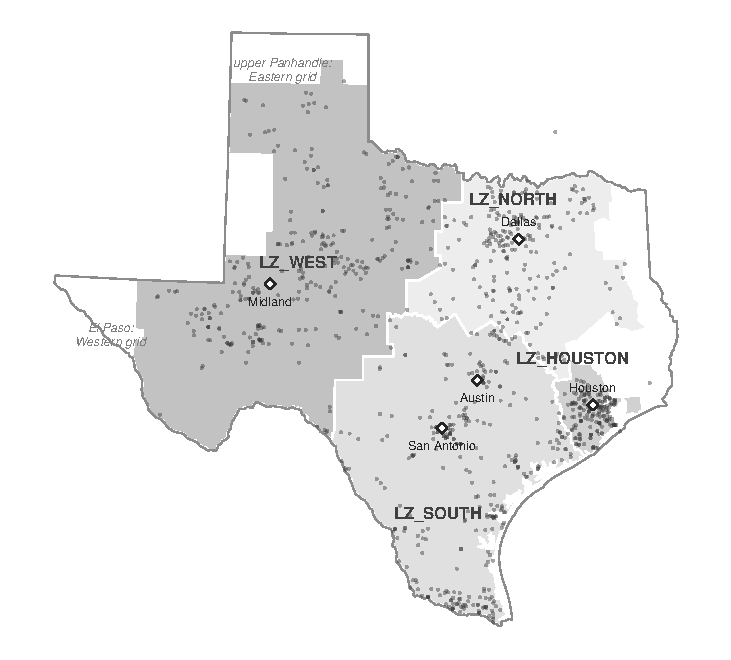
\includegraphics[width=\textwidth]{images/ercot_lz_map}
  \caption{
    ERCOT's four competitive load zones, with generation-side nodes approximated by the 988 grid-connected power plants (dots). The four smaller load zones of the utilities that did not open to retail competition are non-contiguous enclaves within these areas and are not drawn; zone boundaries are approximate, because ERCOT defines zones as sets of electrical buses, not geographic borders. White areas of Texas lie on the Eastern and Western Interconnections, outside ERCOT. Data: EIA-860M, June 2026 \autocite{eia860m2026}. % fig-src: analysis/figures/fig_ch3_lz_map.R (zones: derived third-party GIS tracing of ERCOT's published map, unlicensed re-host, hence "approximate"; outline: Census cb_2023_us_state_20m; plants: EIA-860M BA=ERCO; node/bus coordinates are not published by ERCOT)
  }
  \label{fig:lz-map}
\end{figure}

One of those load zones, \glossaryterm{lz-west}{LZ\_WEST}, appears throughout this book. West Texas has the state's best wind and solar resources, limited transmission out, and, not coincidentally, much of its Bitcoin mining. The result is the most volatile prices in ERCOT: hours of cheap or even negative prices when renewable output exceeds what the wires can carry away, and violent spikes when it does not. During hours with negative prices, generators pay consumers to take power, because subsidized renewables can profitably produce below zero and shutting down costs them more. Chapter~6 quantifies how often.

\section{Scarcity Pricing and the \texorpdfstring{\$5,000}{USD 5,000} Cap}
\label{sec:ordc}

An energy-only market needs administered scarcity pricing, because operating reserves, the safety margin Chapter~2 described, are valuable even in hours when no shortage materializes. From 2014 until the 2025 market redesign, ERCOT implemented this through the \glossaryterm{operating-reserve-demand-curve}{Operating Reserve Demand Curve} (ORDC): a real-time adder to the energy price that grows as available reserves shrink, reflecting the rising probability of losing load \autocite{puct25509}. % src: scarcity pricing mechanism now codified at 16 TAC 25.509; ORDC implemented June 2014 (LOLP x VOLL; VOLL $9,000/MWh in 2021 per potomac2021som p. vi, "the VOLL and HCAP of $9,000"; now set to the HCAP for DAM, $5,000, per ercot2026protocols sec. 4.4.11(1)(a)); under RTC+B the ORDC adder was absorbed into ancillary-service demand curves (see sec:rtcb)
When reserves were plentiful the adder was near zero. When reserves ran thin, the adder pushed prices toward the \glossaryterm{system-wide-offer-cap}{system-wide offer cap}: \$5,000 per megawatt-hour, lowered from \$9,000 after Winter Storm Uri \autocite{ercot2021hcapnotice,puct25509}. Since the redesign of Section~\ref{sec:rtcb}, the ancillary-service demand curves do that pushing from inside the energy price \autocite{ercot2026protocols}. % src: PUCT approved Dec 2, 2021, effective Jan 1, 2022 (ERCOT market notice M-A120721-01); HCAP $5,000 / LCAP $2,000 per 16 TAC 25.509 (b)(6)(A)-(B); still $5,000 as of Aug 2026; since RTC+B ercot2026protocols sec. 4.4.11(1)(a) sets the VOLL used to build the ASDCs to the HCAP for DAM and sec. 6.5.7.3(14)(d) caps bus LMPs, System Lambda and the Real-Time MCPCs at that effective VOLL; real-time energy offers themselves stop at the RTSWCAP, $2,000 (sec. 4.4.11(1) parameter table; sec. 4.4.11(2) rejects offers above it), not printed
A second, smaller adder has ridden on top of it since June 2015, the reliability deployment price adder. When ERCOT keeps the lights on outside the market, by ordering extra generators online or calling on demand response, it adds supply or removes demand and so pushes the price down just when the grid is short; the adder reruns the dispatch as if those actions had not happened and puts the difference back into the price. On average it is small: in 2025 it added \$0.41 per megawatt-hour to the price of energy, against \$0.02 for the ORDC adder. Unlike the ORDC adder, it survived the redesign of Section~\ref{sec:rtcb} \autocite{potomac2015som,potomac2026somercot}. % src: potomac2015som p. 2 (the reliability adder "was implemented on June 25, 2015"; NPRR626 per p. xxv); potomac2026somercot p. 8 ("Actions such as Reliability Unit Commitments (RUCs) and deployment of ERS demand response can artificially lower prices by increasing supply or reducing demand outside the normal market process. The RDPA corrects this suppression by increasing real-time prices when these actions occur"), p. 3 note 2 ("uses the dispatch software to simulate the system lambda without RUCs, deployed load capacity, or certain other reliability actions"), p. 1 ("the ORDC and the RDPA added $0.02 per MWh and $0.41 per MWh, respectively, to the price of energy"; also p. 9), p. A-10 (the RDPA "remains after RTC is implemented", now with separate adders for energy and each AS product); added 2026-10-12 after a review comment that Chapters 5 and 6 and the glossary refer back to an adder this section never introduced

In 2025, a typical ERCOT hour cleared somewhere between \$20 and \$40 per megawatt-hour (the middle half of the year's real-time hours, all eight load zones pooled). % src: analysis/checks/ch3_typical_hour.R console: real-time market, ERCOT MIS 13061 15-min settlement point prices (analysis/data/ercot_rtm15_spp_loadzones_2021on.csv.gz) averaged to clock hours, all eight load zones pooled, calendar 2025: middle half of hours $20.29 to $39.81, median $26.56; holds in 2025; the 2026 partial year comes close ($18.12-$34.83); not in every year: 2024 ran $14.19-$27.74 and 2022 $28.92-$67.43; LZ_WEST alone ran $20.16-$56.74 in 2025
The cap is more than a hundred times that. Prices near the cap arrive rarely, a handful of hours in most years, but for a consumer those hours are catastrophic to buy through and lucrative to avoid. Much of the economic case for miner flexibility in Part III rests on this asymmetry.

Two mechanisms can lower that cap. Since December 2023 the \glossaryterm{emergency-pricing-program}{Emergency Pricing Program} cuts it to \$2,000, for energy and ancillary services alike, once real-time prices have been at \$5,000 for 12 hours within any 24, and holds it there for at least a day and until a day after any emergency ends. And once a hypothetical new peaking plant's earnings above fuel pass \$315,000 per megawatt in a calendar year (three times its yearly building cost), the cap falls to \$2,000 for the rest of that year. Only Uri ever crossed that line, and the commission held off the drop until March 3, 2021, because the low cap then in force was pegged to gas prices and would have come out above \$9,000 \autocite{puct25509,ercot2026protocols,potomac2026somercot,potomac2021som}. % src: puct25509 (c)(1) (EPP "must be activated if the system-wide energy price, as determined by ERCOT, has been at the HCAP for 12 hours within a rolling 24-hour period"), (c)(2) (ECAP = LCAP "for both energy and ancillary service offers"), (c)(3) (in effect until the later of 24 hours after activation or, if ERCOT entered or stayed in emergency operations, 24 hours after it exits them), (b)(2), (b)(4) and (b)(6)(C)-(D) (peaker net margin: RTEP less 10 x the gas index, summed where positive; HCAP "until the peaker net margin during a calendar year exceeds a threshold of three times the cost of new entry", then LCAP "for the remainder of that calendar year"); the EPP is the (c) that PUCT Project 54585 added, effective December 20, 2023 (adoption order: it implements SB 3 sec. 18 "by establishing an emergency pricing program (EPP)"); ercot2026protocols sec. 4.4.11(1)(a)(i) (the trigger is RTM System Lambda plus the Real-Time Reliability Deployment Price Adder for Energy at or above the HCAP for DAM for 12 hours in a rolling 24, on SCED data time-weighted to 15-minute intervals), (1)(a)(ii) and (f), the parameter table (ECAP $2,000, LCAP $2,000, PNM threshold $315,000 per MW-year) and sec. 4.4.11.1(3); potomac2026somercot p. 103 ("three times the CONE over a calendar year, or $315 per kW-year"; "exceeded only once in ERCOT's history, on February 16, 2021, during Winter Storm Uri"); potomac2021som pp. v-vi (the LCAP then "the greater of either $2,000 per MWh or 50 times the natural gas price", which "exceeded the HCAP of $9,000", so the Commission suspended it) and pp. 11-12 and 95 (the suspension "was terminated on March 3, 2021" and the Commission directed ERCOT to resume the LCAP, Project 51812 order of that date); pp. vi and 94-95 say the suspension "occurred" on March 3 and that the Commission "suspended use of the LCAP on March 3"; the date is the reinstatement, per footnote 89 (Project 51812, Order Reinstating Low System-Wide Offer Cap, Mar. 3, 2021) and pp. 11-12
So under the rules in force in 2026 the week of Chapter~2 could not recur at its price, and every value this book measures in that week, in Chapters~6, 7 and~9, was priced under 2021's rules \autocite{puct25509}. % src: puct25509 (c)(1)-(3) (EPP trigger and duration) and (d) ("Beginning January 1, 2026, and every five years thereafter, the commission will review each of the system-wide offer cap programs"); ercot2026protocols sec. 6.5.7.3.1(2)(o) (during ERCOT-directed firm load shed in EEA Level 3 the reliability deployment adder lifts the price to the VOLL used for the RTM ASDCs, which sec. 4.4.11(1)(a)(i) sets to the ECAP while the EPP is active); Uri week at $9,000 for days: chapter 6 sec:indexbill (oxner2021paxtongriddy); the values measured in that week: chapter 6 sec:ownergen (sell option), chapter 7 section "What Standing By Paid" (2021 AS prices), chapter 9 sec:stack-sum and sec:stack-fence (the 2021 ledger year)

\section{Ancillary Services: A First Look}
\label{sec:as-overview}

Alongside energy, ERCOT buys \glossaryterm{ancillary-service}{ancillary services}: standing capabilities that keep the lights on when something breaks. Chapter~2 explained why frequency must be defended second by second; these are the products that defend it. ERCOT's current set has five members \autocite{ercot2025astopics}: % src: ERCOT Trending Topics: Ancillary Services (Dec 2025): Reg-Up, Reg-Down, RRS, ECRS, Non-Spin; ECRS go-live June 9-10, 2023

\begin{itemize}
  \item \glossaryterm{regulation}{Regulation Up and Regulation Down} (Reg-Up, Reg-Down): fast-ramping capacity under ERCOT's automatic control, adjusted on a four-second signal to smooth the continuous wobble between supply and demand.
  \item \glossaryterm{responsive-reserve-service}{Responsive Reserve Service} (RRS): the primary frequency-defense product, deployed automatically when frequency drops. Notably for this book, a large share can be provided by \glossaryterm{load-resource}{load resources}, consumers registered with ERCOT to sell ancillary services; the basic kind sells RRS by tripping offline within half a second on an under-frequency relay \autocite{ercot2026protocols,ercotnog2026}. A miner can hold this role: the ability to disconnect quickly is itself a sellable service. % src: ercot2026protocols sec. 2 (Load Resource: "A Load capable of providing Ancillary Service to the ERCOT System and/or energy in the form of Demand response and registered with ERCOT as a Load Resource"), sec. 3.6.1(1)(a)(iii) (RRS from a CLR with Primary Frequency Response or from a Load Resource on a high-set under-frequency relay) and sec. 3.16(4) (relay loads and FFR together at most 60% of the RRS requirement, the share chapter 7 sec:clr prints); ercotnog2026 sec. 2.3.1.2(6)(a) (total interruption within 30 cycles, 0.5 s, including relay and breaker)
  \item ERCOT Contingency Reserve Service (ECRS): capacity deployable within ten minutes after a contingency such as a large generator trip, introduced in June 2023. Chapter~9 examines the trade-off between selling ECRS and keeping the mine free to stop when electricity costs more than mining earns.
  \item \glossaryterm{non-spinning-reserve}{Non-Spinning Reserve} (Non-Spin): slower backup, capacity that can come online within thirty minutes.
\end{itemize}

What these products pay, and why those payments collapsed after 2021, is the subject of Chapter~7. ERCOT pays for readiness as well as energy, and in the market's eyes a load that can vanish in seconds is a form of readiness.

\section{Paying for the Wires: 4CP}
\label{sec:4cp-intro}

Energy prices do not pay for transmission lines. In ERCOT, transmission costs are allocated by a mechanism with outsized consequences for large consumers: \glossaryterm{4cp}{Four Coincident Peak}, or 4CP. For each summer month (June through September), ERCOT identifies the single 15-minute interval in which system-wide demand peaked. Demand here is a settlement quantity, not the raw load on the control-room screen: ERCOT sums the metered output of its generators, nets off the flows over the DC ties, and excludes the charging of grid-scale batteries entirely \autocite{ercot2026protocols}. % src: Nodal Protocols sec. 9.17.1 (4CP determination: generation-side balance, +DC-tie imports/-exports, +/-Block Load Transfers, minus Wholesale Storage Load); ERCOT notice M-B080124-01 warns the settlement 4CP interval can differ from the interval of highest observed demand; NPRR1188 gray boxes, upon system implementation (early 2027), not printed: sec. 9.17.1(3) (a joint NPRR995 and NPRR1188 box) and (4) also subtract the portion of non-ALR CLR load, and of non-WSL charging load, supplied by co-located generation at sites with a net metering arrangement; sec. 11.1.6(4), for a single-POI Generation Resource site that includes a CLR, counts only the CLR load supplied from the grid in 4-CP and LRS volumes ((c)) but settles the CLR's total load, grid-supplied plus co-located, for energy at the Resource Node ((d)); so a grid-supplied CLR's 4CP is unchanged, and a co-located CLR keeps the netting of any netted load for 4CP and LRS though not for energy (NPRR1188 ERCOT comments, April 4, 2024: co-located CLRs "should receive the same treatment as other types of co-located Load")
A large consumer's share of the following calendar year's transmission costs is then set by its average consumption during exactly those four intervals \autocite{puct25192}. % src: 16 TAC 25.192 (eff. Dec 20, 2022): 4CP data filed by Dec 1 bills transmission for the next year; TDU tariffs (e.g. Oncor) pass through to IDR-metered customers by the customer's own 4CP demand, fixed each Jan 1

Large consumers forecast when the peaks will occur and switch off for them. The metered exposure is one hour a year, four 15-minute intervals, but ERCOT confirms each interval only after the month ends, so in practice loads curtail longer windows across several candidate afternoons. Done well, that discipline can eliminate a transmission bill in the millions. Chapter~8 quantifies what 4CP avoidance is worth per megawatt and how miners chase it.

\section{Real-Time Co-optimization: The 2025 Redesign}
\label{sec:rtcb}

In December 2025, ERCOT switched on its largest redesign since nodal pricing: \glossaryterm{real-time-co-optimization-plus-batteries}{Real-Time Co-optimization plus Batteries} (RTC+B). Before it, ancillary services were bought once, in the Day-Ahead Market, and held fixed; energy was then dispatched around those fixed positions all day. After it, every five-minute SCED run procures energy \emph{and} ancillary services together, repricing both continuously; the old ORDC adder of Section~\ref{sec:ordc} is gone, absorbed into the energy price, and only its curve survives, as the shape the new ancillary-service demand curves are cut from \autocite{ercot2025rtcblive,potomac2026somercot}. % src: ERCOT news release Dec 5, 2025 (go-live); Trending Topics: AORDC used to build AS Demand Curves as inputs to DAM and SCED; ERCOT projects savings exceeding $1B annually. potomac2026somercot p. 2 ("the Operating Reserve Demand Curve (ORDC) Adder, implemented in 2014 and discontinued in December 2025 with the introduction of RTC"), p. 3 ("Since RTC was implemented, shortage pricing has been incorporated into the price of energy rather than functioning as a separate adder"), App. p. A-7 ("These ASDCs effectively replace the ORDC price adder"), App. G ("The ORDC price adder ... was replaced by a set of ASDCs"). The earlier "lives on" wording inverted this and was corrected 2026-09-20

For flexible loads this is a regime change: the value of standing ready is now marked to market every five minutes rather than locked in the afternoon before. The early evidence of what RTC+B does to ancillary prices appears in Chapter~7, and its implications for mining strategy in Chapter~10.

\section{Bitcoin Miners in the ERCOT Market}
\label{sec:miners-ercot}

Each miner deals with ERCOT through a \glossaryterm{qualified-scheduling-entity}{Qualified Scheduling Entity} (QSE). A mine's energy is settled through the QSE of whoever sells it power, and a mine that sells reserves registers as a load resource, whose QSE is a firm it hires or, once it qualifies, itself (Chapter~7) \autocite{ercot2026protocols}. % src: ercot2026protocols (Aug 1, 2026) sec. 16.3.1.1(1) (each LSE applicant "shall designate the Qualified Scheduling Entity (QSE) that will perform QSE functions per these Protocols on behalf of the LSE", with a written statement that the QSE "accepts responsibility for the applicant's transactions"); sec. 3.6.1(2) ("Except for voluntary Load response and ERS, loads participating in any ERCOT market must be registered as a Load Resource") and (3) ("All ERCOT Settlements resulting from Load Resource participation are made only with the Qualified Scheduling Entity (QSE) representing the Load Resource"); sec. 16.5.1.1(1) (each Resource Entity applicant "shall designate" its QSE) and sec. 16.2.3.2(1) ("a Resource Entity serving as its own QSE"), as chapter 6 sec:ownergen and chapter 8 sec:aggregators print
Any load of 75~MW or more at a single site must complete ERCOT's large-load interconnection process, with system studies and a separate approval to energize, before it may draw power \autocite{ercot2025nprr1234}. % src: NPRR1234 (board approved Apr 8, 2025; PUCT approved May 15, 2025; effective Jul 21 / Dec 15, 2025); grew out of the withdrawn NPRR1191
By the end of 2025 ERCOT's large-load program, which takes loads of every industry and not only miners, had about 5,800~MW energized, each site counted at the highest draw it has ever reached. By March 2026 over 9,000~MW, those sites included, held ERCOT's approval to energize \autocite{ercot2026llistatus}. % src: ercot2026llistatus slide 3 (5,768 MW Observed Energized in the 2025 column, defined as projects approved to energize and fully operational, "Represented by all time non-simultaneous peak load consumption"; all project types, with no split by industry anywhere in the deck; the 2025 column's approved total is 6,714 MW, 5,768 energized plus 946 approved but not operational), slide 4 (Approved to Energize by snapshot: 8,786 MW at 2025-12 and 2026-01, 9,042 MW from 2026-02, so the 9,000 MW is dated to the March 2026 deck, not to 2025), slide 5 (approved to energize 5,136 MW LZ_WEST + 3,907 MW other = 9,043 MW, each bar the observed peak plus the remaining approved load) and slide 6 (9,042 MW); the earlier "historically dominated by miners" had no support in the source and was dropped 2026-09-26 (ENERGY-009)
Mining demand alone, by the market monitor's count, peaked near 4,600~MW in 2025 (Chapter~7) \autocite{potomac2026somercot}. % src: potomac2026somercot p. i ("Aggregate demand for crypto-currency mining was approximately 4,600 MW in 2025"), p. 14 (4.6 GW), p. 31 ("peak demand reaching 4,600 MW in 2025"); a different count from the program total above, and neither contains the other: the monitor's figure is mining only, the program's is every industry at 75 MW or more
As Chapter~2 described, during Winter Storm Fern, ERCOT's own analysis credited about 4,100~MW of curtailment to cryptocurrency miners, second only to oil and gas and ahead of every other industry it counted \autocite{ERCOTMonthlyJan2026}. The queue behind them has changed character, though: of the roughly 410~GW of requests from prospective large loads ERCOT was tracking by early 2026, nearly 88~percent were AI data centers and less than 4~percent were mining, the interconnection-side echo of the pivot described in Chapter~1 \autocite{vegas2026senateupdate}. % src: ERCOT CEO Pablo Vegas, Texas Senate B&C testimony, Apr 1, 2026: 410,618 MW tracked by 2030; 87.6% data centers, 3.8% crypto

The rulebook also has words for how a mine sits relative to the grid, and several of them matter later in the book. A \glossaryterm{private-use-network}{Private Use Network} is, in ERCOT's own definition, ``an electric network connected to the ERCOT Transmission Grid that contains Load that is not directly metered by ERCOT (i.e., Load that is typically netted with internal generation)'': a mine built beside a power plant and metered together with it where the pair meets the grid, so that only the net flow is ever settled \autocite{ercot2026protocols}. % src: ercot2026protocols sec. 2 (Private Use Network, verbatim)
ERCOT's definitions also give the 75-megawatt load a name, \glossaryterm{large-load}{Large Load}; if half or more of its demand is ``computational load, such as data centers and cryptocurrency mining facilities,'' it is a \glossaryterm{large-computational-load}{Large Computational Load}, the term the commission's transmission reform in Chapter~8 asks about by name \autocite{ercot2026protocols}. % src: ercot2026protocols sec. 2 (Large Load; Large Computational Load, verbatim)

In 2026 ERCOT began studying its queue of large loads in one batch rather than one by one. In that study a network that pairs a plant with a large load could ask to be treated as a \glossaryterm{withdrawal-limited-private-use-network}{Withdrawal-Limited Private Use Network}: ERCOT models the plant switched off and fixes a hard cap on what the site may draw from the grid. The site may then build up to the plant's output on top of that cap, so a large load that brings its own generation can connect before the transmission upgrades for its full draw are built \autocite{ercot2026protocols,ercotplanningguide2026}. % src: ercot2026protocols sec. 2 (WLPUN: withdrawal limit determined by a system-wide interconnection study conducted by ERCOT) and sec. 3.10.7.3.1 (net Demand at the POI may not exceed the limit; one-minute cure); Planning Guide sec. 9.3.2 (PGRR145, effective July 11, 2026: WLPUN allocated peak Demand capped at the withdrawal limit plus the network's generation)
Chapter~6 prices what such a network is worth to a miner, and what it costs.
The same study offered a second elective route, this one to a large load that brings no plant. A load that asked to be studied as a \glossaryterm{provisional-controllable-load-resource}{Provisional Controllable Load Resource} may draw above the demand the study says the network can serve, up to its full request and with no guarantee that the grid can serve it in real time. It may do so only while it stays registered as a Controllable Load Resource taking ERCOT's dispatch, with its bids capped when a nearby constraint is at risk and no ancillary services to sell. The rules passed with the rest of the batch study in June 2026; the dispatch code behind them is a build ERCOT has ranked for 2027. The window to ask for either route closed in July 2026 \autocite{ercotplanningguide2026,ercot2026protocols}. % src: Planning Guide secs. 9.2.2.1(2) and 9.2.2.2(2) (Form W Part A and Form X due to the Interconnecting DSP or TSP "on or before July 10, 2026", which forwards them to ERCOT "on or before July 24, 2026") and sec. 9.3.1(2)(a) (all Large Load information due to ERCOT by July 24, 2026); Section 9 (effective July 11, 2026) defines only the Batch Zero and legacy procedures and refers to "a future interconnection study process" (sec. 9.2.1(4)) without defining one; Planning Guide secs. 9.2.2.1, 9.3.2 and 9.4.1 (PGRR145: election by Form W; maximum LPC set to the peak Demand that may be served reliably, requested peak Demand approved as MPC contingent on registration; PCLRs exempt from the minimum allocation threshold); Protocols sec. 2 (PCLR definition), sec. 23 Form W (no Real-Time guarantee; PCLRs not eligible to provide Ancillary Services), sec. 6.5.7.3 (dynamic capping of PCLR energy bid curves) and sec. 16.5.5 (de-registration returns the load to its LPC); PUCT approved June 18, 2026, PCLR sections effective upon ERCOT system implementation, priority 2027
In August, at the governor's direction, ERCOT held the study's final verdicts back for an audit of every load's eligibility, due in December. Until that audit and a review of community impact are done, it has stopped approving new data centers and mining sites of 75~MW or more to energize \autocite{ercot2026batchzero}. % src: ercot2026batchzero slides 1 and 3-4 (Governor Abbott's directive of August 3, 2026, a letter per ERCOT market notice M-A080326-01 of the same day; ERCOT's notice paused the Batch Zero study process and delayed final classification, which is now due in December with the Eligibility Verification Report of December 10, 2026, originally August 7, 2026; conditional classification still went to the TSPs on September 3, 2026, as chapter 10 sec:outlook-grid prints; approvals to energize data centers and virtual currency mining facilities of 75 MW or greater paused until the verification and audit and the community impact review, whose report is also due December 10, are complete; impact on the study timeline "TBD", originally April 9, 2027 under Planning Guide sec. 9.3.1(2)(b))

The market rules of this chapter explain \emph{why} Texas, and West Texas in particular, accumulated so much Bitcoin mining. Published day-ahead prices make tomorrow's expensive hours visible in advance. Locational pricing hands the cheapest, most volatile prices to the region with the most stranded renewable energy. Scarcity pricing makes the worst hours expensive enough that avoiding them is a business. Ancillary services pay for interruptibility itself, and a load that disappears for four well-chosen quarter-hours a summer walks away from its share of the transmission bill. In August 2023, a record month, Riot Platforms booked \$24.2~million for reselling at spot the power its fixed-price contracts had bought and \$7.4~million from ERCOT's demand-response programs, while the 333 bitcoin it mined were worth roughly \$9.5~million; on the real-time index the same pauses would have bought no power and booked no resale credit (Chapter~6) \autocite{riot2023august,riot10k2024}. % src: Riot press release Sep 6, 2023 (SEC 8-K Ex. 99.1; release and table re-read 2026-09-27): "a new monthly record for Power and Demand Response Credits, totaling $31.7 million in August" (the two components are printed, not the total, which the release rounds: 24.2 + 7.4 = 31.6); table: Power Credits $24.2M, fn "Power curtailment credits received from the Company's ability, under its long-term power contracts, to sell power back to the ERCOT grid at market-driven spot prices"; Demand Response Credits $7.4M, fn "Credits received from participation in ERCOT demand response programs"; "Power Credits and Demand Response Credits for July and August 2023 are estimates"; 333 BTC produced, 300 sold for $8.6M net at $28,617 average net price -> 333 x 28,617 = $9.53M (at the August average price implied by Riot's "approximately 1,136 Bitcoin" equivalence, 31.7M / 1,136 = $27,905, $9.29M); the credits are gross, counted before the bitcoin the curtailed hours would have mined, which no public source gives, so no net figure is printed; the old "the flexibility paid more than three times the mining" (31.7 / 9.53 = 3.3x) was retired 2026-09-27 (EXEC-021) because it read as a net payoff; riot10k2024 Note 20 (Rockdale PPA: 345 MW of long-term, fixed-price power, with the election not to use it and to sell it instead, as the opening of chapter 6 prints); index equivalence: chapter 6 sec:arbitrage ("the contract price cancels out of the decision") and chapter 9 sec:stack-contract (S19j Pro pause option $1.41M on the real-time index and $1.41M under a fixed $27 contract with sell-back, 2025); each resold MWh is credited P - F, the price less the fixed price, which is (P - V) + (V - F), and only the option P - V is index-equivalent, the V - F being the margin mining would have earned anyway (chapter-6.tex sec:arbitrage, the Riot credits sentence, riot10k2024: "the difference in the market power price and our fixed power price"), so on the index the same pauses are worth less than the $24.2M; the $7.4M of demand-response credits is paid the same on either contract; until 2026-09-27 this line said the resale was "worth the same" on the index, and the clause saying so is gone

Miners can earn money through ERCOT's incentives for flexible consumption without anyone needing to believe in bitcoin. How much that flexibility earns, hour by hour and program by program, is the business of the rest of this book.
